% mnras
% \documentclass[fleqn,useAMS,usenatbib]{mnras}

% apj
%\documentclass[iop, twocolappendix, appendixfloats, numberedappendix, apj]{emulateapj}
\documentclass[iop, twocolappendix, appendixfloats, numberedappendix, apj]{hackemulateapj}
%\documentclass{emulateapj}

%=====================================================================
% CUSTOM: PACKAGES, MACROS & SETTINGS
%=====================================================================
% packages for figures
\usepackage{graphicx,todonotes}

% packages for symbols
\usepackage{latexsym,amssymb}

% AMS-LaTeX package for e.g. subequations
\usepackage{amsmath,morefloats}
\usepackage[backref,breaklinks,colorlinks,citecolor=blue]{hyperref}
\usepackage{natbib,graphicx,amsmath,subfigure,color,xcolor}
%\usepackage{natbib,graphicx,amsmath,subfigure,color,xcolor,hyperref}
\usepackage{verbatim}
\usepackage{threeparttable}

%\usepackage{lineno}
%\linenumbers

\topmargin-1cm

\graphicspath{{figures/}}

\newcommand\notedo[1]{\todo[color=yellow, inline, size=\small]{To do:#1}}
\newcommand\notewrite[1]{\todo[color=orange, inline, size=\small]{To write: #1}}
\newcommand\noteask[1]{\todo[color=cyan, inline, size=\small]{To ask: #1}}
\newcommand\notecontrib[1]{\todo[color=green, inline, size=\small]{Contributors: #1}}
\newcommand\esstodo[1]{\todo[color=yellow, inline, size=\small]{ESS: #1}}
\newcommand{\ess}[1]{\textcolor{red}{[ESS: \bf #1]}}
\newcommand{\mrb}[1]{\textcolor{purple}{[MRB: \bf #1]}}


\newcommand{\vecg}{\mbox{\boldmath $g$}}
\newcommand{\vece}{\mbox{\boldmath $e$}}
\newcommand{\veck}{\mbox{\boldmath $k$}}
\newcommand{\vecQ}{\mbox{\boldmath $Q$}}
\newcommand{\vecF}{\mbox{\boldmath $F$}}
\newcommand{\vecD}{\mbox{\boldmath $D$}}
\newcommand{\matR}{\mbox{$\bf R$}}
\newcommand{\matC}{\mbox{$\bf C$}}
\newcommand{\bnab}{\boldsymbol{\nabla}}
\newcommand{\bnabg}{\boldsymbol{\nabla_g}}
\newcommand{\galsim}{\texttt{GALSIM}}
\newcommand{\ngmix}{\texttt{ngmix}}
\newcommand{\nnsim}{\texttt{nsim}}
\newcommand{\snr}{$S/N$}
\newcommand{\sn}{$S/N$}
\newcommand{\coadd}{{\rm coadd}}
\newcommand{\desreq}{$4\times 10^{-3}$}
\newcommand{\lsstreq}{$2\times 10^{-3}$}

\newcommand{\mcal}{\textsc{metacalibration}}
\newcommand{\mdet}{\textsc{metadetection}}
\newcommand{\Mcalshort}{\textsc{metacal}}
\newcommand{\Mcal}{\textsc{Metacalibration}}
\newcommand{\Mdet}{\textsc{Metadetection}}
\newcommand{\vest}{\mbox{\boldmath $e$}}
\newcommand{\est}{e}
\newcommand{\mcalR}{\mbox{\boldmath $R$}}
\newcommand{\mcalRS}{\mbox{\boldmath $R_S$}}
\newcommand{\gest}{\mbox{\boldmath $\hat \gamma$}}
\newcommand{\vecgam}{\mbox{\boldmath $\gamma$}}

\newcommand{\sx}{\textsc{Source Extractor}}

\newcommand{\bfd}{\textsc{BFD}}

\newcommand{\vonkarman}{{von K\'arm\'an}~}


%\setuphead[section][before={\testpage[2]}]

%mnras
%\title[\Mdet]{\Mdet: Mitigating Shear-dependent Object Detection Biases with \Mcal}

%\author[Sheldon et~al.]{Erin Sheldon$^1$, Matthew R. Becker$^2$,
%Niall MacCrann$^{3,4}$, Michael Jarvis$^5$
%  \\$^1$Brookhaven National Laboratory, Bldg. 510, Upton, NY 11973, USA
%  \\$^2$High Energy Physics Division, Argonne National Laboratory, Lemont, IL 60439, USA
%  \\$^3$Center for Cosmology and Astro-Particle Physics, The Ohio State University, Columbus, OH 43210, USA
%  \\$^4$Department of Physics, The Ohio State University, Columbus, OH 43210, USA
%  \\$^5$Department of Physics and Astronomy, University of Pennsylvania, Philadelphia, PA 19104, USA
%}


% apj
\shorttitle{\Mdet}
\shortauthors{Sheldon, Becker, MacCrann, Jarvis}

\begin{document}
% mnrad
% \date{Draft \today}

% mnras
%\maketitle

% apj
%\title{\Mdet: Mitigating Shear-dependent Object Detection Biases with \Mcal}
\title{Metadetection: Mitigating Shear-dependent Object Detection Biases with Metacalibration}

\author{Erin S. Sheldon}
\affil{Brookhaven National Laboratory, Bldg 510, Upton, New York 11973, USA}
\author{Matthew R. Becker}
\affil{High Energy Physics Division, Argonne National Laboratory, Lemont, IL 60439, USA}
\author{Niall MacCrann}
\affil{Center for Cosmology and Astro-Particle Physics, The Ohio State University, Columbus, OH 43210, USA}
\affil{Department of Physics, The Ohio State University, Columbus, OH 43210, USA}
\author{Michael Jarvis}
\affil{Department of Physics and Astronomy, University of Pennsylvania, Philadelphia, PA 19104, USA}


\begin{abstract}

    \Mcal\ is a new technique for measuring weak gravitational lensing shear
    that is unbiased for isolated galaxy images.  In this work we test \mcal\
    with overlapping, or ``blended'' galaxy images.  Using standard \mcal, we
    find a few percent bias for galaxy densities relevant for current surveys,
    and that this bias increases with increasing galaxy number density.  We
    show that this bias is not due to blending itself, but rather to
    shear-dependent object detection. If object detection is shear independent,
    no deblending of images is needed, in principle.  We demonstrate that
    detection biases are accurately removed when including object detection in
    the \mcal\ process, a technique we call \mdet.  This process involves
    applying an artificial shear to images of small regions of sky, and
    performing detection and measurement on the sheared images in order to
    calculate a shear response.   We show that the method works up to
    second-order shear effects even in highly blended scenes.  However, because
    the space between objects is sheared coherently in this process, the
    accuracy of \mdet\ is ultimately limited by how closely this matches images
    in real data, where some, but not all galaxies in an image are sheared
    coherently.  We find that even in the worst case scenario, in which
    the space between objects is completely unsheared, the bias is at
    most a few tenths of a percent for future surveys.  We show that the
    primary technical challenge for \mdet, deconvolution using a spatially
    varying point-spread-function, does not result in a significant bias for
    typical imaging surveys.  Finally, we discuss additional technical
    challenges that must be met in order to implement \mdet\ for real surveys.


    %This process involves applying an artificial shear to images
    %of small regions of sky, and performing detection and measurement on the
    %sheared images. The ensemble response of the measurements to the applied
    %shear is then calculated, with measurements now including the process of
    %detection, and this response is used to calibrate the final shear estimate.
    %We show that the primary technical challenge for \mdet, deconvolution using
    %a spatially varying point-spread-function, does not cause in a significant
    %bias for typical imaging surveys.  Finally, we discuss the physical limits
    %of \mdet's accuracy.  The key assumption behind \mdet\ is that the entire
    %region of sky under consideration, which we are free choose to be small, is
    %sheared, including the space between objects, as opposed to only the images
    %of the objects.  In the real universe, lensing over cosmological distances
    %produces a combination of these scenarios.  We test the worst case scenario
    %for \mdet, in which only images of objects are sheared, and find the bias
    %is at most a few tenths of a percent for future surveys.  We discuss
    %additional technical challenges that must be met in order to implement
    %\mdet\ for real surveys.

\end{abstract}

\section{Introduction}

Recently developed methods to estimate weak gravitational lensing shear can in
principle provide calibration at the 0.1\% level or better, sufficient for the
requirements of future weak lensing surveys \citep[e.g.,][]{huterer2006}.  At
the time of writing, two methods have demonstrated sufficient accuracy without
reliance on calibration from simulations, including rigorous mathematical
formalisms to deal with selection effects:  the \bfd\ method
\citep{BernBFD2016} and the \mcal\ method \citep{HuffMcal2017,SheldonMcal2017}.
However, the existing tests of \bfd\ and \mcal, while stringent, did not
include an important aspect of the real universe: the images of objects overlap
on the sky and thus the light from separate objects is ``blended'' \citep[for
discussion of blending effects see, e.g.,][]{DawsonBlending2016}.

\mcal\ can, in principle, be used calibrate any shear measurement biases, even
those associated with blending.  However, we will show below that there is a
particular calibration bias associated the process of detecting objects in the
presence of blending, and this is not addressed in naive implementations of
\mcal. This bias is especially large for ambiguous detections on highly blended
images and thus poses a challenge for future lensing surveys in which
blending will be important \citep{DawsonBlending2016}.

At this stage it is worthwhile to define exactly what we mean by object
detection.  For isolated objects, object detection is closely related to the
detection of regions of an image with pixel values above some threshold; this
is perhaps the traditional meaning of the word detection. But when objects
overlap on the sky, whether due to physical association or chance projection,
there may be an additional desire to determine how many objects there are in
each detected region. This may be desirable, for example, when assigning a
redshift distribution to a set of detections.  We associate this process with
object detection.  We reserve the term ``deblending'' to specifically mean the
process of assigning a fraction of the light in each pixel to each detected
object, which may or may not be a feature of the object detection.  In this
work, for the sake of brevity, we will use the terms ``detection'' and ``object
detection'' interchangeably.

In the weak shear regime, the lensing mapping is one-to-one and preserves
surface brightness \citep{SchneiderBook92}. For such a mapping, object
detection need not be shear dependent. For example, an object detection
algorithm that identifies connected regions in an image with pixel values above
a threshold will not in principle be shear dependent.  This is because the
topology of the contours, or the number of closed contours, at a given surface
brightness will not change under a shear, due to the preservation of surface
brightness and the one-to-one nature of the mapping.  However, in real
observations the image resolution is degraded by a point-spread-function (PSF)
due to the atmosphere, telescope optics and detector. In this case the overlap
of objects, and also the topology of contours of a given surface brightness,
does depend on shear because the PSF convolution occurs after the shear
mapping.  This effect is demonstrated in Figure~\ref{fig:toy}.  Thus the simple
threshold object detection method described above will manifest a
shear-dependent object detection bias. Note this effect is present even in the
absence of pixel noise.

\begin{figure*}
    \begin{center}
        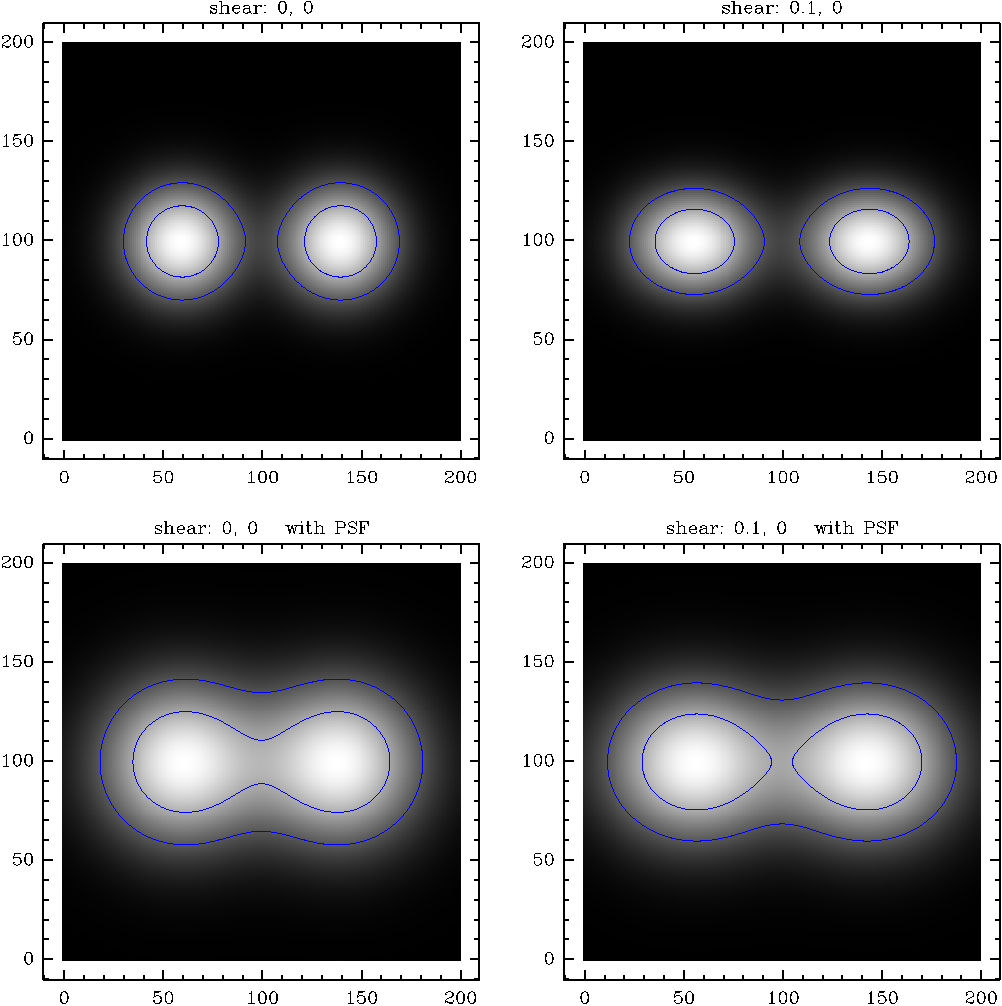
\includegraphics[width=\textwidth]{figures/toy.pdf}

        \caption{ Toy example of shear-dependent object detection in the presence of
        a PSF.  In panel (a) two objects are present, convolved by a PSF with no
        shear.  Contours represent constant brightness.  In panel (b) the objects
        are sheared by $\gamma = (0.0, 0.1)$ {\em after} the PSF convolution.  The
        contour levels are the same as panel (a).  In this case the inner contours
        for the two objects overlap before and after application of the shear. This
        is a general property of the shear transformation in the weak regime:
        surface brightness is preserved under shear, and because the mapping is
        one-to-one, the topology is also preserved. In panel (c) the shear is
        applied {\em before} the PSF convolution, which mimics real sky images. In
        this case the inner contours do not overlap after shearing, and two objects
        may be detected rather than one.  For case (c) an object detection
        algorithm that identified connected regions above a threshold as a single
        object would manifest a shear-dependent object detection bias.
        \label{fig:toy} }
    \end{center}

\end{figure*}

Common object detection schemes in use today, such at those in \sx\
\citep{Bertin96} and the HST/LSST pipelines \citep{BoschHSC2018,BoschLSST2018}
are based on thresholding, similar to the simple approach described above but
differing in complexity and efficiency. The effective threshold used to divide
regions into separate objects in these codes is not a simple threshold above
noise, but is rather a relative quantity.  This is demonstrated clearly for
\sx\ in \cite{Bertin96} Figure~2.  Thus we would expect object detections
produced by such a code to also manifest shear dependence. A simple local peak
finder, run on a smoothed image, has similar properties\footnote{An open question,
which we will not address in this work, is whether it is possible to derive a
shear-independent object detection algorithm  in the presence of a PSF and a
detector with finite spatial resolution.  Such an algorithm would in principle
eliminate the shear-dependent object detection biases explored in this work.}

Published implementations of \mcal\
\citep[e.g.,][]{HuffMcal2017,SheldonMcal2017}, when used with the common object
detection schemes discussed above, are expected to exhibit shear-dependent
object detection biases. These implementations of \mcal\ work by applying
artificial shears to small ``postage stamp'' images, extracted from a larger
image, for objects found during an {\em independent} object detection step, run
before the application of \mcal, followed by a calculation of the response of
an ellipticity measurement to the applied shear. This independent object
detection will already manifest a shear-dependent object detection bias, and
thus any shear applied when running \mcal\ does not properly reflect the full
response to shear.

This shear-dependent object detection bias is a type of selection effect.
Corrections for selection effects in a static catalog were already derived in
\cite{SheldonMcal2017}, but that formalism implicitly assumes that the base
catalog itself is unaffected by selection effects.  Similarly, that formalism
cannot work for objects near the object detection threshold, even for isolated
objects, because the object detections needed for the corrections will, by
definition, not be present in the catalog.

As we will demonstrate, object detection effects can be naturally incorporated
into \mcal\ by shearing somewhat larger images, rather than small postage
stamps, and re-running the object detection algorithm on each of the sheared
images. In this process, ellipticity measurement biases, selection effects and
object detection are all accounted for simultaneously. We call this technique
\mdet.

Calibration with simulations is an alternative route being explored by the
community \citep[see, e.g.,][]{KIDS450shear,HSCY1shear}.  The idea is to use an
uncalibrated ellipticity measurement, which can manifest a large shear bias
(of order 10\%) and  unknown selection effects.  The final shear
measurements are then calibrated, including selection effects, using a
simulation that matches the data as closely as possible.  Ultimately \mdet\ may
have some remaining biases that must be calibrated with simulations.  Our goal
in developing this algorithm is to make these biases as small as possible,
sub-percent as opposed to 10 percent, which we expect will greatly reduce the
sensitivity of the final calibration to small inaccuracies in the simulation.

The paper is laid out as follows. In Section~\ref{sec:sims}, we describe our
simulation and analysis techniques. In Section~\ref{sec:detbiases}, we study
the effects of object detection on shear measurements with \mcal.
In Section~\ref{sec:mitigate}, we describe \mdet\ which combines \mcal\ with
an object detection algorithm in order to mitigate the shear biases from object
detection. We also discuss the physical limits of \mdet\ there.
In Section~\ref{sec:psfvar}, we study the effects of the PSF variation on \mdet.
Finally, we conclude in Section~\ref{sec:conc}.

\section{Analysis and Simulation Techniques}
\label{sec:sims}

In this section, we describe our object simulation and measurement techniques.
In all cases, we used the \galsim\ \citep{GALSIM2015} software package to
generate images, perform convolutions etc. We used the \texttt{SEP} \citep{sep}
Python wrapper of the \sx\ software package \citep{Bertin96} for
source detection as needed. Finally, we made extensive use of \ngmix
\footnote{\url{https://github.com/esheldon/ngmix/}} for object measurement and
the \mcal\ implementation.

\subsection{\textsc{Metacalibration}}
\label{sec:mcal}

\mcal\ is a general technique that computes the linear response of image
measurements to an applied shear using only the observed image.  For a small
applied shear $\boldsymbol{\gamma}$, we can expand a measurement $\boldsymbol{e}$ as
\begin{eqnarray}
\boldsymbol{e} & \approx & \left.\boldsymbol{e}\right|_{\gamma=0} +
                           \left.\frac{\partial \boldsymbol{e}}{\partial\boldsymbol\gamma}\right|_{\gamma=0} \boldsymbol\gamma +
                           O(\boldsymbol\gamma^2)\nonumber\\
               & \equiv  & \left.\boldsymbol{e}\right|_{\gamma=0} +
                           \boldsymbol{R} \boldsymbol\gamma +
                           O(\boldsymbol\gamma^2)
\end{eqnarray}
where $\boldsymbol{R}$ is the response matrix of the image measurement
at zero applied shear, $R_{ij}=\partial e_i /\partial \gamma_j$, with $i$ and
$j$ taking all combinations of the two shear components.  The measurement
$\boldsymbol{e}$ can be, for example,  an ellipticity measurement, and in what
follows we will use the term ellipticity without loss of generality.

We estimate the response using a numerical, finite-difference derivative
\begin{equation}
R_{ij} \approx \frac{e_i^{+} - e_i^{-}}{\Delta\gamma_j}\ .
\end{equation}
where $R_{ij}$ is the estimated response of the measurement to shear and
$\Delta\gamma_j = 2 \gamma_j$ is the difference between two applied shears,
$\pm \gamma_j$, with $\gamma_j$ a small shear, usually of order 0.01. The
quantity $e_i^{+/-}$ is the $i$-th ellipticity component measured on an image
sheared with $\pm\Delta\gamma_j$.  The $e_i^{+/-}$ used in the finite
differences measured on artificially sheared images \citep{SheldonMcal2017},
the creation of which requires careful handling of the PSF and other
observational effects.  Note that as the estimated responses per-object are
quite noisy, they must be averaged over many images/objects in order to
estimate the response of a set of images/objects to a shear.
We will expand this method to include object detection in section
\ref{sec:mitigate}.

We will focus on detection biases in this work, but there are a number of steps
in the image processing that are shear dependent: detection, centroiding,
ellipticity measurement, flux measurement, etc.  In this sense, the \mdet\
method will measure the response of all image manipulations and measurements to
an applied, constant shear.

\subsection{Multi-object Fitting Deblending}

Multi-object Fitting (MOF) deblending is a technique employed by the Dark
Energy Survey to account for blending of objects when performing image
measurements \citep{DESY1cat}. It is representative of a set of techniques that
involve fitting models to images for a list of preexisting detections. The
model fit is then used directly to form a flux measurement or indirectly by
using it to approximately remove the light of the neighboring objects in the
image before further processing.

In this work, we used an \ngmix\ based MOF
algorithm\footnote{\url{https://github.com/esheldon/mof/}}. It is an improved
version of the MOF fitter used in \cite{DESY1cat} which is
both more stable and faster. It uses a linear combination of a De Vaucouleurs'
\citep{devauc1948} profile and exponential profile. The profiles are
constrained to be cocentric, coelliptical, and to have a fixed one-to-one size
ratio.  The relative amplitude of the two profiles, the fraction of the total
flux in the De Vaucouleurs' profile, is a free parameter and is allowed to vary
outside of the range [0, 1]. Finally, to process a large number of objects, we
followed \citet{DESY1cat} and broke them up into associated groups.  These
groups of objects were then simultaneously fit using a least-squares loss
function.

\subsection{Galaxy Pair Simulations}
\label{sec:sims:pairs}

In order to isolate the effects of detection easily, we employed a simulation
setup consisting of two galaxies with a variable separation between them.  We
varied the separation of the objects in order to carefully tune the effects of
blending.

The simulated galaxies were each a combination of a bulge component, modeled as
a De Vaucouleurs' profile \citep{devauc1948} and disk component modeled as an
exponential. The fraction of light in the bulge was random and ranged uniformly
between 0.0 and 1.0. The disk ellipticity was drawn from the distribution
presented in \cite{ba14}, equation 24, with ellipticity variance set to 0.20,
with a random orientation. The bulge was given the same orientation as the disk
but with ellipticity set to the disk ellipticity times a random number drawn
uniformly between 0.0 and 0.5. The half-light radius of the disk
$r_{50}^{\mathrm{disk}}$ was set to a uniform random draw between 0.4 and 0.6
arcsec. The half-light radius of the bulge was a random draw between $0.4
r_{50}^{\mathrm{disk}}$ and $0.6 r_{50}^{\mathrm{disk}}$. The bulge was shifted
from the center of the disk within a radius 0.05$r_{50}^{\mathrm{disk}}$ and in
a random direction. The light of the disk was divided between a smooth
component and a set of simulated ``knots of star formation'', represented by
point sources placed randomly with the same exponential distribution as the
disk.  Between 1 and 50 knots were placed, such that the fraction light in the
knots ranged between 0.4\% and 20\%. The total flux and noise were set such
that the signal-to-noise ratio ranged uniformly between 25 and 35.  The models
were convolved by a PSF modeled as a Moffat \citep{Moffat1969} profile with
$\beta=2.5$ and full with at half maximum 0.9 arcseconds, and rendered into an
image with pixel scale 0.263 arcseconds.

We rendered two of these randomly generated galaxies in an image, with
separation ranging from 1.0 and 4.0 arcsec. The pair was situated such that the
line between the pair had a uniform random orientation relative to the
coordinate axes. Each object was given an additional random dither within a
pixel. The galaxies were treated as transparent, such that the value in a pixel
was equal to the total sum from both galaxies plus noise. Example images are
shown in Figure~\ref{fig:pairs}

\begin{figure*}
    \begin{center}
        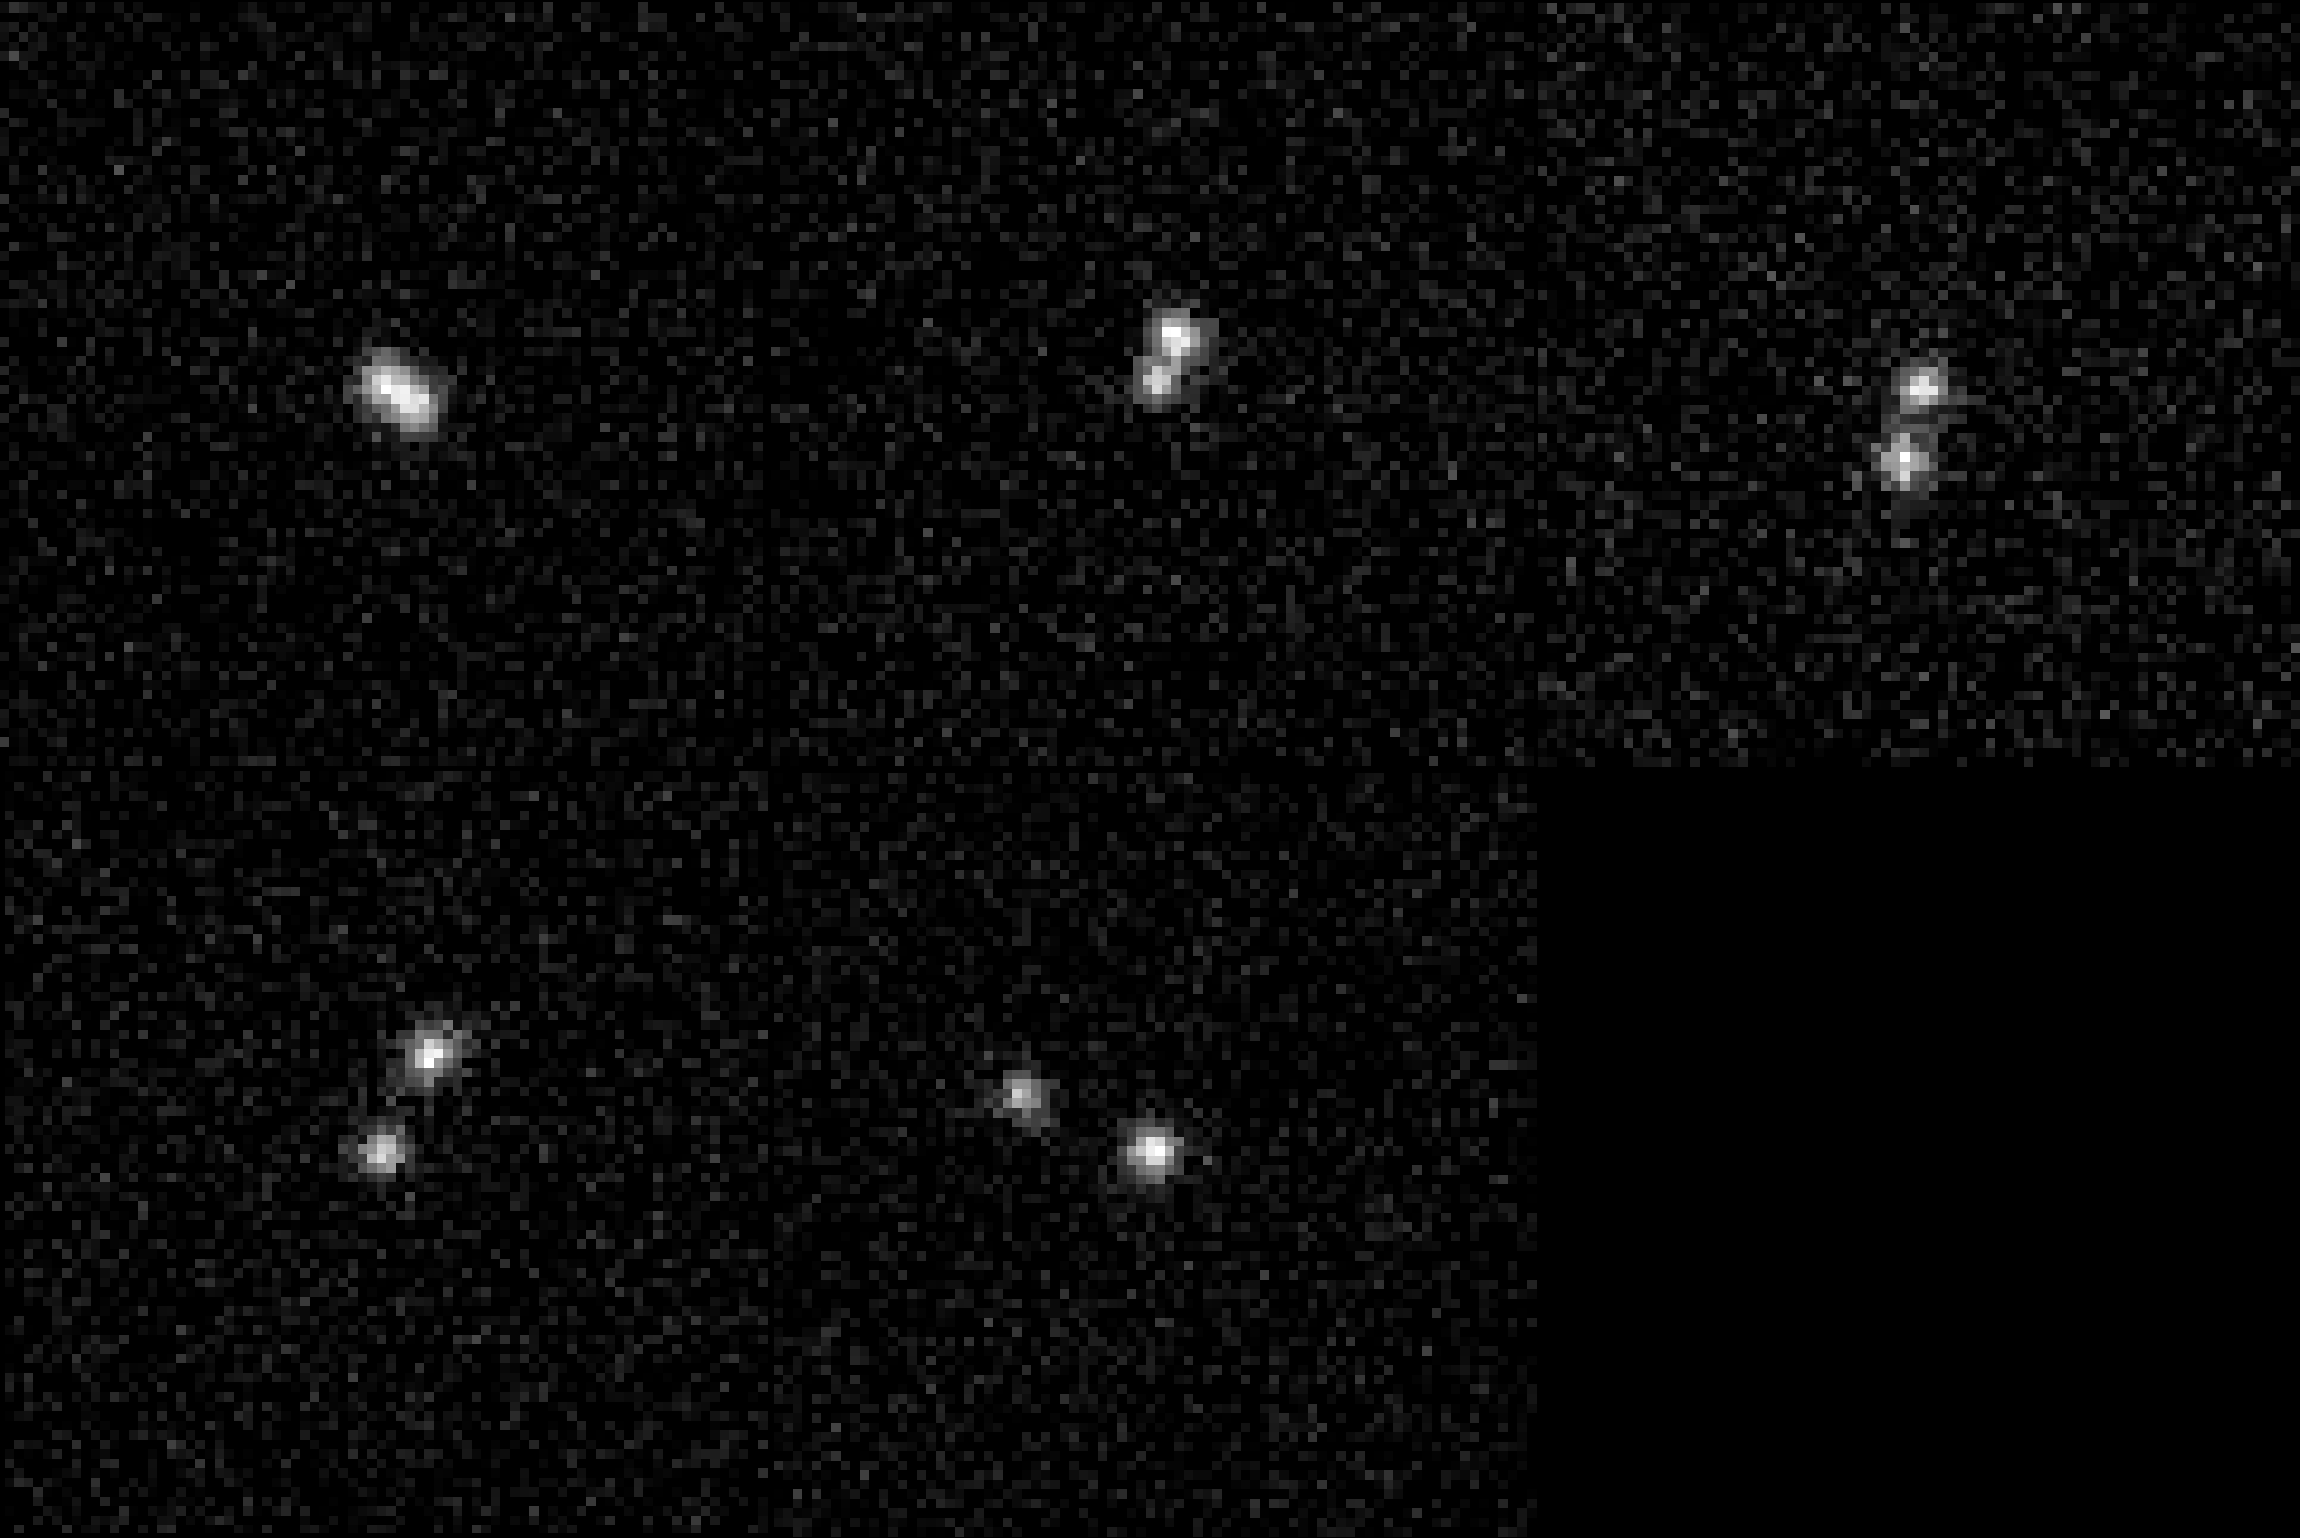
\includegraphics[width=\textwidth]{figures/bdk-comb.png}
        \caption{Example images of simulated galaxies used for the pair tests
        presented in section \ref{sec:sims:pairs}.  From left to right in the top row,
        the separations are 1.0, 1.5, 2.0 arcsec. From left to right in the bottom row the
        separations are 3.0 and 4.0 arscec. The pixel scale is 0.263 arcsec.
        \label{fig:pairs}}
    \end{center}
\end{figure*}

\subsection{Simulations with Representative Galaxy Density and Noise}
\label{sec:sims:realgals}

We used the
\texttt{WeakLensingDeblending}\footnote{\url{https://github.com/LSSTDESC/WeakLensingDeblending}.
Note this package uses Galsim for all object models and rendering.} package to
generate image simulations with realistic galaxy densities and pixel noise for
both the DES and LSST surveys.

We generated images in the r-, i-, and z-bands with an effective depth that is
roughly equivalent to full 5 and 10 year coadd image for the DES and LSST
respectively. For our primary tests, we neglected the effects of PSF variation
and used a constant PSF per-band with the typical (expected) seeing for each
survey ($\sim\!1$ arcsec and $\sim\!0.8$ arcsec respectively). We tested
variable PSFs separately, as discussed in \S \ref{sec:psfvar}.  For the DES
image simulations, we modified the settings slightly such that the effective
exposure time was equivalent to ten 90 second exposures. The depths of the LSST
images were set to match those assumed by the \texttt{WeakLensingDeblending}
package for the 10 year survey, although note the modifications below. In all
simulations a shear of $\gamma_1 = 0.02$ was used.

We made two additional modifications to the simulations produced by this
package.  The galaxy models and PSFs were generated using the
WeakLensingDeblending package, using its internal survey settings and object
catalogs.  But rather than using the package to render into an image, we
rendered them separately so that we could control whether the full scene was
sheared, including the space between objects, or just the objects were sheared
(the only mode supported by WeakLensingDeblending).

We also multiplied the density of input sources by a factor of 0.45 and a
factor of 0.4 for the DES-like and LSST-like simulations, respectively, in
order to produce a realistic number density of detected sources. We also
performed tests with the unmodified input catalog for the LSST-like
simulations, in order to test with an extreme density. The detected source
densities in these three simulations were approximately 35 per square arcmin
for DES year 5, 75 per square arcmin for LSST year 10, and 140 per square
arcmin with the unmodified source catalog for the LSST-like simulations.
Example images for each survey are shown in Figure~\ref{fig:simimages}.

\begin{figure*}
    \begin{center}
        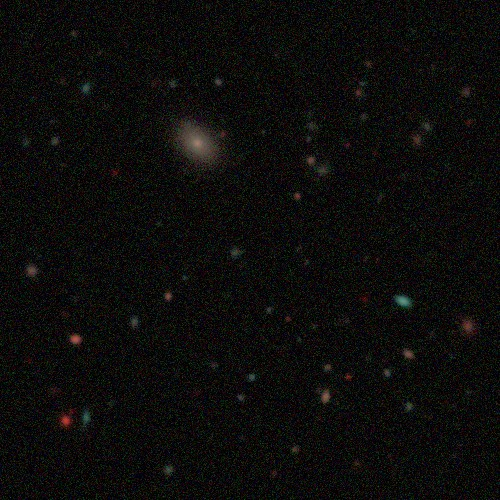
\includegraphics[width=0.9\columnwidth]{figures/des_gri.jpg}
        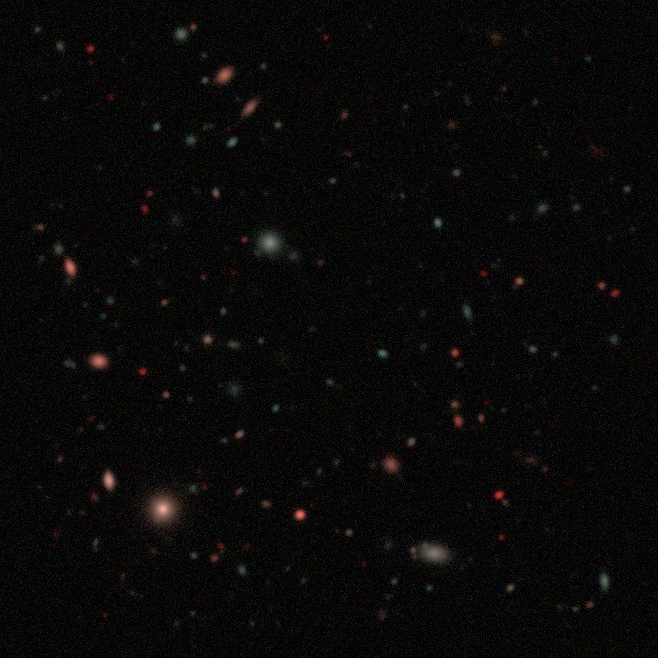
\includegraphics[width=0.9\columnwidth]{figures/lsst_gri.jpg}
        \caption{
            Example images from the DES (left) and LSST (right) simulations. Each
        multicolor, $gri$-band image is approximately $\sim\!2.2$ arcmin on a side. The
        DES images have a pixel scale 0.263 arcsec and a PSF FWHM of $\sim\!1$ arcsec.
        The LSST images have a pixel scale of 0.2 arcsec and a PSF FWHM of $\sim\!0.8$
        arcsec.
        \label{fig:simimages}}
    \end{center}
\end{figure*}


\subsection{Measuring Shear Biases}

We report our results in terms of the standard parameterization of shear
measurement biases \citep[see, e.g.,][]{heymans2006}

\begin{equation} \label{eq:m}
g \equiv c + (1 + m)\gamma
\end{equation}
where $g$ is the recovered shear, $c$ is the additive bias, and $m$ is the
multiplicative bias. Below we report only $m$, but we have found that $c$ is
consistent with zero in all cases.

We used the technique of \citet{pujol2019} to reduce the noise on measurements
of $m$ in our simulations.  This technique works as follows. We generated pairs
of images with identical galaxy and noise properties, but with opposite true
shears applied $\gamma_{\pm}$ (we use a scalar notation because the shear
was only applied in one component).  For each pair of simulations, we calculate the mean
ellipticity and mean response.  We then calculate ensemble means $\langle e_\pm \rangle$
and $\langle R \rangle = ( \langle R_+ \rangle + \langle R_- \rangle)/2$ over all such
pairs of images, and form a difference of the overall recovered shear that
partially cancels noise:
\begin{equation}
    \gamma_{est} = \frac{ \langle e_+ \rangle - \langle e_- \rangle}{2 \langle R \rangle},
\end{equation}
We then calculated $m$ using equation \ref{eq:m}, $\gamma_{est}$ and the true
input shear.  We estimated the errors on the mean $m$ using bootstrap
resampling of the set of image pairs, repeating the computation of $m$ for each
bootstrap sample. We employed a similar procedure for $c$, except that we used
the average of the two estimated shears so that any additive biases common to
both simulations do not cancel. In all  cases we measured $m$ using the
1-component of the shear and $c$ with the 2-component of the shear, though we
have found this choice not to matter in explicit testing.

\section{Shear-dependent Detection Biases}\label{sec:detbiases}

In this section, we present results from a variety of specialized simulation
setups to elucidate the role of detection biases in \mcal\ shear measurements.
We first examine shear measurement on pairs of galaxies at various separations.
We then study detection biases in DES- and LSST-like simulations with
realistic galaxy densities and pixel noise. We find in all cases that object
detection imparts a non-negligible shear measurement bias. As we will show in
\S \ref{sec:mdetpairs}, we can correct this bias by including detection in the
\mcal\ process, even if no explicit deblending (division of light between
objects) is performed.

\subsection{Bias in Simulations of Galaxy Pairs}

We tested \mcal\ with MOF deblending using the galaxy pair simulation presented
in \S \ref{sec:sims:pairs}. We used \sx\ for object detection, with settings
matching those used for DES year 5 survey reductions (DES Collaboration, in
prep.)\footnote{We have created a software package to run detection with DES
year 5 settings, using the sep \sx\ wrapper
\url{https://github.com/esheldon/sxdes}}.  We got similar results using a
simple local peak finder for
detection\footnote{\url{https://github.com/esheldon/peaks}}.  We also saw
similar levels of bias with and without performing deblending using MOF.

The multiplicative bias $m$ is shown in Figure~\ref{fig:pairbias} as a function
of the pair distance. For a large separation of 4 arcsec, two objects were
detected in essentially all cases, but as the separation was decreased the
detection became more ambiguous, with only one object detected in some cases.
At 1.5 arcsec separation the detection was most ambiguous, with two objects
detected in half the cases. As the separation was decreased further, one object
was detected more often than two, and at 1.0 arcseconds only one object was
detected in essentially all cases.  For close separations the blend is
unrecognized but the detection is unambiguous, in the sense that the
detection algorithm consistently finds one object.

In the cases where the detection is unambiguous, at close and far separations,
there is no bias in the recovered shear.  But the bias increases as the
detection becomes more ambiguous. The maximum bias occurs at 1.5 arcsec
separation, where two objects are detected in half the cases, the separation of
maximum ambiguity.

\begin{figure}
    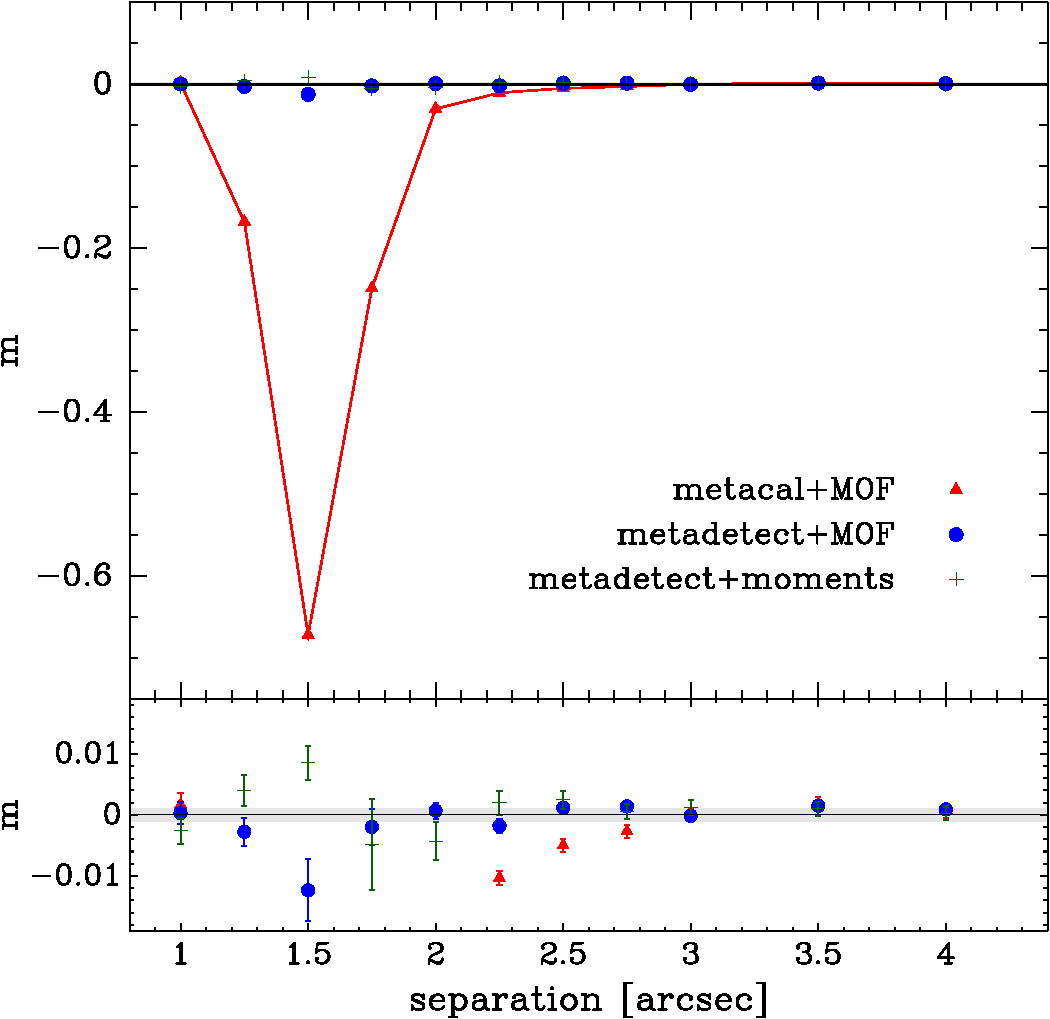
\includegraphics[width=\columnwidth]{figures/pairs-mc-bdkpair.pdf}

    \caption{Mean multiplicative shear bias measured for pairs of simulated
    galaxies (see \S \ref {sec:sims:pairs} for details) at various separations.  At
    each separation, a large number of trials was generated with random
    orientations of the pair.  At 4.0 arcsec separation, two objects were
    detected in all cases.  At 1.5 arcseconds two objects were detected in half
    the cases.  At 1.0 arcsec a single object was detected in all cases.  Red
    triangles represent standard \mcal\ with MOF deblending for modeling all
    detected objects.  Blue circles represent \mcal+MOF with detection included
    as part of the process.  Green pluses represent \mcal\ with detection
    included but without deblending, and using simple weighted moments without
    PSF correction as the shear estimator. Very large biases are seen for
    standard \mcal+MOF as detection becomes ambiguous, for example at 1.5
    arcsec separations.  When detection is included in the \mcal\ process the
    biases are greatly reduced.  The bias is reduced even in the case where no
    deblending was performed and no PSF correction or detailed object modeling
    were performed.  This indicates that a majority of the bias is due to
    shear-dependent detection, not light blending or details of the object
    modeling.
    \label{fig:pairbias}}

\end{figure}

The correspondence between detection ambiguity and shear bias is a hint that
the bias is caused by shear-dependent detection. Next, we test with simulations
of DES- and LSST-like surveys and show explicitly that by turning object
detection off, we can eliminate these detection biases.


\subsection{Bias in Simulations with Representative Galaxy Density and Noise}

The results for simulations with representative galaxy density and noise are
shown in Table~\ref{tab:shearmeas}.  \mcal\ with MOF deblending and \sx\
detections results in large biases, $\sim-3\%$, for a full five year
DES-like survey. Simulations of LSST-like surveys demonstrate somewhat larger
biases, and a simulation with double the LSST galaxy density shows a very large
bias\footnote{The bias numbers here are fairly noisy, but it is interesting to
note that the bias for LSST year 10 is not very much larger than DES year 5,
despite the fact that the galaxy density is about twice as high.  This may be
partly due to the better resolution of the LSST images: the area of the LSST
PSF 60\% smaller than DES PSF.  Thus the images of
small galaxies, at fixed density, will overlap less in LSST images than they do
in DES images}.  Note, we see similar biases when no deblending is performed.

% raw outputs
% DES mcal+MOF
%                                              s2n: 10
% # of sims: 497756
% m       : -0.036147 +/- 0.004863
% c [1e-4]: -0.624614 +/- 1.764896
%                                              s2n: 15
% # of sims: 488295
% m       : -0.023056 +/- 0.004427
% c       : -0.000203 +/- 0.000208
%                                              s2n: 20
% # of sims: 472679
% m       : -0.014961 +/- 0.004202
% c       : -0.000133 +/- 0.000227
%
% LSST mcal+MOF
%                                              s2n: 10
% # of sims: 469550
% m       : -0.034729 +/- 0.002272
% c [1e-4]: -0.186440 +/- 0.848381
%                                              s2n: 15
% # of sims: 469549
% m       : -0.030558 +/- 0.001999
% c [1e-4]: -0.442153 +/- 0.904867
%                                              s2n: 20
% # of sims: 469548
% m       : -0.025855 +/- 0.001802
% c [1e-4]: -0.354317 +/- 0.965168
%
% ==> run_galwldeblend_DES_shearscene/condor_shear_meas.txt <==
% s2n: 10
%     # of sims: 118989
%     m [1e-3]: 0.253494 +/- 0.878401
%     c [1e-4]: -0.082117 +/- 0.306233
% s2n: 15
%     # of sims: 118989
%     m [1e-3]: -0.847165 +/- 0.704490
%     c [1e-4]: -0.210065 +/- 0.345075
% s2n: 20
%     # of sims: 118989
%     m [1e-3]: 0.237638 +/- 0.614585
%     c [1e-4]: -0.138857 +/- 0.408659
%
% ==> run_galwldeblend_LSST_shearscene/condor_shear_meas.txt <==
%                                                  s2n: 10
%     # of sims: 10000000
%     m [1e-3]: 0.839101 +/- 0.609534
%     c [1e-4]: -0.253958 +/- 0.236264
%                                                  s2n: 15
%     # of sims: 9999990
%     m [1e-3]: -0.011541 +/- 0.472899
%     c [1e-4]: -0.092792 +/- 0.245059
%                                                  s2n: 20
%     # of sims: 9999869
%     m [1e-3]: 0.416105 +/- 0.394588
%     c [1e-4]: -0.176120 +/- 0.270438
%
% ==> run_galwldeblend_DES/condor_shear_meas.txt <==
% s2n: 10
%     # of sims: 48431641
%     m [1e-3]: -4.229170 +/- 0.872680
%     c [1e-4]: 0.233764 +/- 0.236895
% s2n: 15
%     # of sims: 46324536
%     m [1e-3]: -5.166098 +/- 0.645108
%     c [1e-4]: -0.003570 +/- 0.263022
% s2n: 20
%     # of sims: 43766867
%     m [1e-3]: -5.887744 +/- 0.567673
%     c [1e-4]: -0.149850 +/- 0.286801
%
% ==> run_galwldeblend_LSST/condor_shear_meas.txt <==
%                                                  s2n: 10
%     # of sims: 10000000
%     m [1e-3]: -1.489893 +/- 0.733162
%     c [1e-4]: -0.302429 +/- 0.249726
%                                                  s2n: 15
%     # of sims: 9999992
%     m [1e-3]: -1.327159 +/- 0.641900
%     c [1e-4]: -0.020227 +/- 0.265990
%                                                  s2n: 20
%     # of sims: 9999898
%     m [1e-3]: 0.102487 +/- 0.531214
%     c [1e-4]: -0.291314 +/- 0.266207

\begin{table*}
  \centering
    \begin{threeparttable}
  \caption{
    Multiplicative biases in weak lensing simulations for various shear
    measurement techniques. In all cases, the simulations use realistic
    galaxy ellipticities, galaxy sizes and noise for the given survey. For measurements using standard \mcal\ with
    MOF deblending, a cut of $T/T_{PSF} > 0.5$ was also applied. Measurements with
    \mdet\ and moments used a size cut of $T/T_{PSF} > 1.2$. In the case of \mdet\ with moments,
    no deblending corrections are applied and the moments are a simple weighted moment
    with no PSF correction.}
  \label{tab:shearmeas}

  %\begin{tabular}{|l|l|l|c|c|}
  \begin{tabular}{lllcc}
    \hline
    \noalign{\vskip 1mm}
    Simulation & Method & Full Scene Sheared? & \snr\ Cut & m \\
    \noalign{\vskip 1mm}
    \hline
    \noalign{\vskip 1mm}

    %\hline
    \multicolumn{5}{c}{metacal+MOF - full scene sheared}\\
    \noalign{\vskip 1mm}
    \hline
    \noalign{\vskip 1mm}
    DESY5   & metacal+MOF & yes & \snr$ > 10$ & $-0.036 \pm 0.005$  \\
    DESY5   & metacal+MOF & yes & \snr$ > 15$ & $-0.023 \pm 0.004$  \\
    DESY5   & metacal+MOF & yes & \snr$ > 20$ & $-0.015 \pm 0.004$  \\
    \noalign{\vskip 1mm}
    \hline
    \noalign{\vskip 1mm}
    LSSTY10  & metacal+MOF & yes & \snr$ > 10$ & $-0.035 \pm 0.002$  \\
    LSSTY10  & metacal+MOF & yes & \snr$ > 15$ & $-0.031 \pm 0.002$  \\
    LSSTY10  & metacal+MOF & yes & \snr$ > 20$ & $-0.026 \pm 0.002$  \\
    \noalign{\vskip 1mm}
    \hline
    \noalign{\vskip 1mm}
    LSSTY10 2$\times$ dens. & metacal+MOF & yes & \snr$ > 10$ & $-0.082 \pm 0.005$  \\
    LSSTY10 2$\times$ dens. & metacal+MOF & yes & \snr$ > 15$ & $-0.067 \pm 0.005$  \\
    LSSTY10 2$\times$ dens. & metacal+MOF & yes & \snr$ > 20$ & $-0.062 \pm 0.004$  \\
    \noalign{\vskip 1mm}
    \hline
    \noalign{\vskip 1mm}

    %\hline
    \multicolumn{5}{c}{metadetect+moments - full scene sheared}\\
    \noalign{\vskip 1mm}
    \hline
    \noalign{\vskip 1mm}
    DESY5   & metadetect+moments & yes & \snr$ > 10$ & $+0.00025 \pm 0.00088$  \\
    DESY5   & metadetect+moments & yes & \snr$ > 15$ & $-0.00085 \pm 0.00070$  \\
    DESY5   & metadetect+moments & yes & \snr$ > 20$ & $+0.00024 \pm 0.00061$  \\
    \noalign{\vskip 1mm}
    \hline
    \noalign{\vskip 1mm}
    LSSTY10  & metadetect+moments & yes & \snr$ > 10$ & $+0.00084 \pm 0.00061$  \\
    LSSTY10  & metadetect+moments & yes & \snr$ > 15$ & $-0.00001 \pm 0.00047$  \\
    LSSTY10  & metadetect+moments & yes & \snr$ > 20$ & $+0.00042 \pm 0.00039$  \\
    \noalign{\vskip 1mm}
    \hline
    \noalign{\vskip 1mm}
    LSSTY10 2$\times$ dens. & metadetect+moments & yes & \snr$ > 10$ & $+0.00047 \pm 0.00043$  \\
    LSSTY10 2$\times$ dens. & metadetect+moments & yes & \snr$ > 15$ & $-0.00002 \pm 0.00034$  \\
    LSSTY10 2$\times$ dens. & metadetect+moments & yes & \snr$ > 20$ & $+0.00019 \pm 0.00028$  \\
    \noalign{\vskip 1mm}
    \hline
    \noalign{\vskip 1mm}

    %\hline
    \multicolumn{5}{c}{metadetect+moments - individual objects sheared}\\
    \noalign{\vskip 1mm}
    \hline
    \noalign{\vskip 1mm}
    DESY5                 & metadetect+moments & no & \snr$ > 10$ & $-0.0042 \pm 0.0009$  \\
    DESY5                 & metadetect+moments & no & \snr$ > 15$ & $-0.0052 \pm 0.0006$  \\
    DESY5                 & metadetect+moments & no & \snr$ > 20$ & $-0.0059 \pm 0.0006$  \\
    \noalign{\vskip 1mm}
    \hline
    \noalign{\vskip 1mm}
    DESY5 2$\times$ dens. & metadetect+moments & no & \snr$ > 10$ & $-0.0029 \pm 0.0006$  \\
    DESY5 2$\times$ dens. & metadetect+moments & no & \snr$ > 15$ & $-0.0017 \pm 0.0005$  \\
    DESY5 2$\times$ dens. & metadetect+moments & no & \snr$ > 20$ & $-0.0023 \pm 0.0005$  \\
    \noalign{\vskip 1mm}
    \hline
    \noalign{\vskip 1mm}
    LSSTY10                 & metadetect+moments & no & \snr$ > 10$ & $-0.0015 \pm 0.0007$  \\
    LSSTY10                 & metadetect+moments & no & \snr$ > 15$ & $-0.0013 \pm 0.0006$  \\
    LSSTY10                 & metadetect+moments & no & \snr$ > 20$ & $+0.0001 \pm 0.0005$  \\
    \noalign{\vskip 1mm}
    \hline
    \noalign{\vskip 1mm}
    LSSTY10 2$\times$ dens. & metadetect+moments & no & \snr$ > 10$ & $-0.0047 \pm 0.0006$  \\
    LSSTY10 2$\times$ dens. & metadetect+moments & no & \snr$ > 15$ & $-0.0035 \pm 0.0004$  \\
    LSSTY10 2$\times$ dens. & metadetect+moments & no & \snr$ > 20$ & $-0.0029 \pm 0.0004$  \\
    \noalign{\vskip 1mm}
    \hline
  \end{tabular}

    \end{threeparttable}
\end{table*}


% raw outputs w/ 2x density
% DES mcal+MOF
% s2n: 10
%     # of sims: 49499
%     m       : -0.066781 +/- 0.009613
%     c       : -0.000055 +/- 0.000371
% s2n: 15
%     # of sims: 49496
%     m       : -0.050463 +/- 0.008567
%     c       : 0.000271 +/- 0.000416
% s2n: 20
%     # of sims: 49476
%     m       : -0.037302 +/- 0.007727
%     c       : 0.000201 +/- 0.000449

% LSST mcal+MOF
% s2n: 10
%     # of sims: 49014
%     m       : -0.082423 +/- 0.005180
%     c       : -0.000245 +/- 0.000192
% s2n: 15
%     # of sims: 49014
%     m       : -0.066753 +/- 0.004539
%     c       : -0.000173 +/- 0.000197
% s2n: 20
%     # of sims: 49014
%     m       : -0.062331 +/- 0.004279
%     c       : -0.000094 +/- 0.000210

% DES shear scene
% s2n: 10
%     # of sims: 9997419
%     m       : 0.000161 +/- 0.000857
%     c       : -0.000011 +/- 0.000034
% s2n: 15
%     # of sims: 9982020
%     m       : 0.000407 +/- 0.000786
%     c       : -0.000036 +/- 0.000039
% s2n: 20
%     # of sims: 9928501
%     m       : 0.000814 +/- 0.000754
%     c       : -0.000013 +/- 0.000044

% LSST shear scene
% s2n: 10
%     # of sims: 9996600
%     m       : 0.000472 +/- 0.000433
%     c       : -0.000024 +/- 0.000018
% s2n: 15
%     # of sims: 9996600
%     m       : -0.000015 +/- 0.000339
%     c       : -0.000003 +/- 0.000017
% s2n: 20
%     # of sims: 9996600
%     m       : 0.000190 +/- 0.000284
%     c       : -0.000012 +/- 0.000018

% DES no shear scene
% s2n: 10
%     # of sims: 40134959
%     m [1e-3]: -2.855179 +/- 0.585444
%     c [1e-4]: -0.096807 +/- 0.186636
% s2n: 15
%     # of sims: 40087901
%     m [1e-3]: -1.676965 +/- 0.513632
%     c [1e-4]: -0.225602 +/- 0.207248
% s2n: 20
%     # of sims: 39905852
%     m [1e-3]: -2.314589 +/- 0.475903
%     c [1e-4]: -0.178327 +/- 0.231775

% LSST no shear scene
% s2n: 10
%     # of sims: 9999000
%     m       : -0.004659 +/- 0.000559
%     c       : -0.000024 +/- 0.000018
% s2n: 15
%     # of sims: 9999000
%     m       : -0.003514 +/- 0.000430
%     c       : -0.000003 +/- 0.000018
% s2n: 20
%     # of sims: 9999000
%     m       : -0.002873 +/- 0.000367
%     c       : -0.000022 +/- 0.000019


In order to unpack the source of the bias in this case, we compared two
different \mcal\ shear measurements. The first was performed on a catalog of the true
source positions using a fixed 1.2 arcsecond Gaussian weighted moment
ellipticity measurement. The second employed \mcal\ with the same ellipticity
measurement, but using \sx\ detections rather than the true object positions. We
found that while the first \mcal\ shear measurement is unbiased
($-0.0011\pm0.0012$), the second exhibits a bias of
$-0.058\pm0.001$.\footnote{The simulations with the true source positions are
computationally slow because they involve measurements on all sources, even
ones which are undetectable. Thus we were unable to decrease the errors on the
multiplicative bias below $\sim0.1\%$. However, for simulations with round,
exponential, high signal-to-noise objects only, we have found that \mcal\ with
the true source positions and a weighted moment has bias ($0.00033 +/-
0.00009$) in the presence of blending, consistent with the bias expected due to
the breakdown of the weak lensing approximation.} Note that this ellipticity
measurement makes no corrections for object blending, but in the case where we
use the true object positions, it is still unbiased. Thus we have demonstrated
that given a set of true source locations, \mcal\ is not sensitive to
blending.\footnote{In practice, we have found that when using \mcal\ with true
detections and more complex ellipticity measurements, for example using a
non-linear model fit, biases can enter at the few tenths of a percent level.
Thus whether \mcal\ is unbiased when using true detections does depend on the
technique used to measure ellipticities on the sheared \mcal\ images.}

This set of tests also demonstrates explicitly that source detection can cause
significant shear measurement biases even for techniques which are robust to
blending. The source detection biases probably originate from multiple causes,
but one of those causes is certainly the merging or splitting of object detections
in a way that is shear dependent, as illustrated with the toy example in
Figure~\ref{fig:toy} and the galaxy pair tests above.

\section{Mitigating Shear-dependent Detection Biases} \label{sec:mitigate}

In the previous section, we demonstrated that source detection is a significant
source of bias in shear measurements with \mcal. Here we show we can
mitigate this bias by including source detection in the
\mcal\ process.

We generated relatively large images, $\sim$ 2 arcminutes on a side, and applied
\mcal\ directly to the full image using the PSF at the center of the image for
deconvolutions.  We performed object detection on each of the five artificially
sheared images (see \S \ref{sec:mcal}) using \sx.  We then
made measurements in postage stamps around each detection in each image using a
non-PSF corrected, Gaussian-weighted moment.  These five catalogs were then
combined into a single estimate for the shear by computing the
average shear response for the image
\begin{eqnarray}
\langle \boldsymbol\gamma \rangle &\approx& \langle \boldsymbol{R}\rangle^{-1}\langle\boldsymbol{e}\rangle\nonumber\\
\langle R_{ij}\rangle &=& \frac{\langle e_i^{+}\rangle - \langle e_i^{-}\rangle}{\Delta\gamma_j}
\end{eqnarray}
where the equation for the response above is for a single shear component. We term this
process \mdet.

Note that the averages above are over the {\it catalogs} from running source
detection and ellipticity measurement on differently sheared images. This is in
effect the ``total derivative'' response, shown in section 3 of
\cite{SheldonMcal2017}, without any attempt to split the response into the
shear response and selection response using the chain rule.  Shear responses
for individual detected objects, as used in both \cite{SheldonMcal2017} and
\cite{HuffMcal2017}, were not calculated.  Doing so would require matching the
lists of detections found on the different sheared images, so that finite
differences for each object could be formed.  This act of matching would
introduce the very shear-dependent object detection biases we wish to
calibrate.  We will discuss the implications of this fact for the analysis of
imaging surveys in \S \ref{sec:wavg}.

\subsection{Results for Simulated Galaxy Pairs}
\label{sec:mdetpairs}

In Figure~\ref{fig:pairbias} we show results for the simulations of galaxy
pairs, now including detection in the \mcal\ process. The blue filled circles
represent the case where deblending is performed using MOF. The green plus
signs represent the case where no deblending was performed. For the case
without deblending,  we further simplified the process: we calculated
simple weighted moments at the position determined by \sx\ using a fixed weight function
with full-width at half maximum 1.2 arcsec, without any correction for the PSF.

In both cases the bias is greatly reduced, with significant bias seen only at
the special separation of 1.5 arcsec, where the two objects are detected as one
object by \sx\ in half of the cases. This demonstrates that the bias we see is
not primarily due to the process of deblending itself, but rather
shear-dependent detection effects. The remaining biases at 1.5 arcsec tend to
be different sign for the deblended and non-deblended cases, which shows there
is a qualitative difference in how the two measurements respond to the shear.
As we will show below, we find no significant net bias for more realistic DES
and LSST-like images where the typical separation of galaxies is not at a
special value of maximum detection ambiguity.

\subsection{Results for Simulations with Representative Galaxy Density and Noise}
\label{sec:res:constpsf}

We show results for DES-like and LSST-like surveys in Table~\ref{tab:shearmeas}.
We have used a constant PSF and constant shear for these simulations. We find
that in all cases our \mdet\ shear measurements are unbiased up to
second-order shear effects \citep[we expect a bias of a few parts in 10000 for shears
of 0.02, see][]{SheldonMcal2017}. This conclusion holds despite the extensive blending
of the object images and the large source detection effects we documented
above. They also meet or exceed the requirements for analyzing an LSST-like survey
\citep[e.g.,][]{huterer2006}. Finally, note that we have also shown results for an
LSST-like survey where the number density of objects is approximately twice that
expected from the actual survey.  Even at these higher densities we find
no increase in the shear bias.

\subsection{Testing the Physical Assumptions Behind \mdet}
\label{sec:mdetphys}

Here we address a key physical assumption made by \mdet, namely that the space
between all objects is sheared coherently.   With \mdet\ we shear the entire
image, so the space between object is sheared as well as their shapes, and this
is completely coherent across the image.  In \S \ref{sec:res:constpsf} we
showed that, when the shear in the simulation matches this procedure exactly,
we calculate the response accurately.

But real data typically contains images of objects sheared by different amounts
at different redshifts, and can be thought of as a sum of a series of constant,
but differently sheared images.  In such an image, the shearing is not
completely coherent.  Variable shear itself is not a source of bias for \mdet;
the formalism presented in \citep{SheldonMcal2017} recovers the mean shear or
other ensemble statistic for a population.  But because the shearing of the
space between objects in real data is not completely coherent, we may expect
that the part of the \mdet\ response associated with {\em detection} is
slightly biased.

\begin{comment}
each small
region of sky that is processed (say 2 arcminutes on a side) has been
transformed by a constant shear.  In such an image, the full scene is sheared,
including the space between objects, not just the shapes of the objects. This
shearing of the space between all objects matches the \mdet\ shearing steps
exactly, and thus allows us to calibrate the mean shear from a set of such
images to high precision, as shown in \S \ref{sec:res:constpsf}.  However, real
data will typically contain images of objects sheared by different amounts at
different redshifts, and can be thought of as a sum of a series of constant,
but differently sheared images.
\end{comment}

\begin{comment}
But This image would not exactly match the \mdet\
assumption that the entire scene has experienced a single constant shear, and
thus we might expect some residual bias in the shear calibration. Note that
non-constant shear in the sense that objects will experience shears is not in
itself a source of bias, because it is the mean shear, or other ensemble
statistic, that is recovered by the formalism \citep{SheldonMcal2017}.
\end{comment}

In Figure~\ref{fig:toynoscene} we show a toy example, similar to
Figure~\ref{fig:toy}, demonstrating the extreme and unphysical case of two
objects that are in line-of-sight projection but sheared completely
independently.  We did not allow the space between objects to be sheared. The
contours of constant surface brightness differ less after shear than those
shown in \ref{fig:toy}.  This is intuitive, because the relative separation
between objects does not change.  The \mdet\ process of shearing the full
image, which does move the positions of objects, will over-predict the response
in this case.

In general, we expect a larger bias due to this effect for surveys with more
object blending, which scales with object density and PSF size.  To test these
expectations, we created a set of simple simulations in which we sheared the
shapes of objects, but not the space between objects.  We simulated round
galaxies with exponential light distributions and a half-light-radius of 0.5
arcsec. We then tested the accuracy \mdet\ shear recovery under varying
conditions, namely with either 45 objects per square arcmin or 140 objects per
square arcmin, and with either a 0.9 arcsec Gaussian PSF or a 1.1 arcsec
Gaussian PSF. Our results are reported in Table~\ref{tab:nssres} and confirm
these expectations. However, we don't expect these results to be representative
of realistic scenarios.


\begin{figure*}
    \begin{center}
        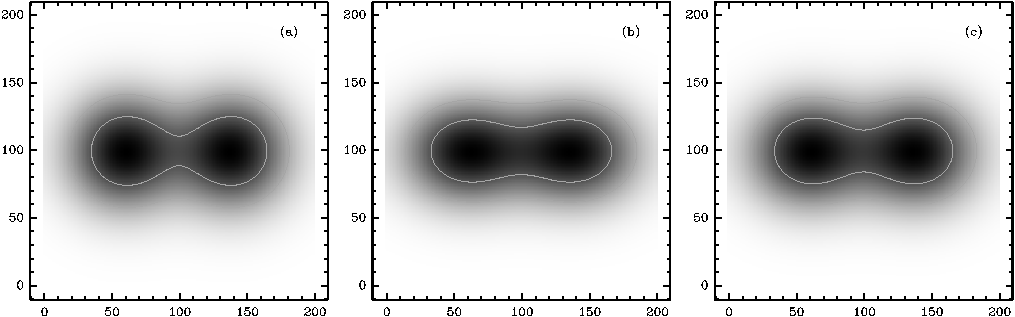
\includegraphics[width=\textwidth]{figures/toy-no-full-scene.pdf}

        \caption{Same as Figure~\ref{fig:toy} but the shear was applied to the
        objects without shearing the space between them. This models the extreme
        and unphysical case where two objects are in line-of-sight projection but
        sheared completely independently.  The contours changed less after shearing
        in this case as compared to the contours in Figure~\ref{fig:toy}.  This
        case differs from the \mdet\ process, in which the entire image is sheared,
        including the space between images.  \label{fig:toynoscene} }
    \end{center}

\end{figure*}


\begin{table}
  \centering
  \begin{threeparttable}
  \caption{
    Multiplicative biases in weak lensing simulations for various source
    densities and PSF sizes when the space between objects is not sheared. See
    Section~\ref{sec:mdetphys} for details. In all cases, the simulations use a
    population of round, exponential objects with a half-light-radius of 0.5
    arcsec. We used a DES-like pixel scale of 0.263 arcsec, applied \mdet\
    with a simple weighted moment with no PSF correction, and then finally
    used a size cut of $T/T_{PSF} > 1.2$ for the measurements.}
  \label{tab:nssres}
  \begin{tabular}{llc}
    \noalign{\vskip 1mm}
    \hline
    \noalign{\vskip 1mm}
    Galaxy Density & PSF FWHM & m \\
    \noalign{\vskip 1mm}
    \hline
    \noalign{\vskip 1mm}
    45 $\mathrm{arcmin}^{-2}$  & 0.9 arcsec & $-0.00087 \pm 0.00016$ \\
    140 $\mathrm{arcmin}^{-2}$ & 0.9 arcsec & $-0.00247 \pm 0.00015$ \\
    45 $\mathrm{arcmin}^{-2}$  & 1.1 arcsec & $-0.00136 \pm 0.00022$ \\
    140 $\mathrm{arcmin}^{-2}$ & 1.1 arcsec & $-0.00443 \pm 0.00021$ \\
    \noalign{\vskip 1mm}
    \hline
  \end{tabular}
  \end{threeparttable}
\end{table}

In order to obtain an upper bound on this effect for real surveys, we made a
simple modification to our simulations with realistic galaxy density and noise.
When building them, rather than shearing the full scene to impart the true
shear to the image, we sheared each object individually and then added it to
the image, without any change in the object position. This modification leaves
the space between objects unsheared, which is maximally different from what
happens during the \mcal\ image shearing process.

Results for our more realistic survey simulations are in the bottom rows
of Table~\ref{tab:shearmeas}. We found small residual biases in this case,
of order $\sim-0.3\%$. While the fact that we find more bias for a DES-like
survey than an LSST-like survey can be explained by the large PSFs in the
DES-like survey and the smaller pixel scale in the LSST-like survey, some of
the DES-like results are puzzling. In particular, the trend with object density
in the DES-like surveys appears to be opposite our naive expectation. We do
not fully understand this effect. While predicting the expected level of this
bias for experiments such as such as DES and LSST is essential, it is beyond
the scope of this work.

\section{Handling PSF Variation}
\label{sec:psfvar}

In order to apply \mdet\ to a real, multi-band, multi-epoch survey like the DES
or LSST, we must address realistic levels of PSF variation, missing data, and
non-trivial WCS transformations. We will address missing data and WCS issues in
a future work, currently in preparation. Here we address the issue of PSF
variation, which is technically the most challenging because \mdet\ requires
deconvolution by the PSF over relatively large regions of sky.

The deconvolution of a spatially varying PSF formally requires a spatially
varying kernel, the implementation of which would be computationally
challenging.  We instead adopted efficient FFTs for deconvolution, which require
a constant kernel.  For this kernel, we chose to use the PSF associated with
the center of the final coadd image, which is thus systematically wrong at
other locations and will necessarily produce a bias in the recovered shear.
However, we will show that the image coadding process used in a realistic
multi-epoch survey results in a more uniform PSF in the final coadd, and
sufficiently reduces associated biases.

For these simulations, we used a simple population of galaxies that have
exponential profiles with a half light radius of 0.5 arcsec. All of the objects
were round and were rendered at a signal-to-noise ratio greater than 20. These
simulations had very low ellipticity noise and so could reach a high precision
with a relatively small number of images. We created the images for the
simulation by coadding a number of images with random, variable PSFs.  \mdet\
was then performed using the coadd of PSF models from the input images, with
the PSF from each input image generated at the location of the center of the
final coadd.

In order to place an upper bound on this effect, we created a variable PSF
model that had significantly more variation than we expect in real data. See
Appendix~\ref{app:pspsf} for details.  Using a single PSF realization from
Appendix~\ref{app:pspsf}, without coadding, we found a multiplicative bias of
$-0.0065 +/- 0.00044$.  However, when coadding thirty of these models, which is
the expected number of epochs for three bands in the final DES data set, we
found a multiplicative bias of only $-0.00035 +/- 0.00037$.  For LSST many more
epochs will be available for coadding.   While this test is not conclusive, we
expect that in a realistic survey scenario, PSF variation will not be a
fundamental limitation for \mdet.

\section{Implications for the Analysis of Imaging Surveys} \label{sec:wavg}

The fact that five separate catalogs must be used without any attempt at
matching them (see \S \ref{sec:mitigate}), has implications for using \mdet\ in
the analysis of surveys.  Typically a single reference or ``gold'' sample of
objects is constructed and used for all subsequent calculations, such as
calculating redshift distributions.  With \mdet, multiple such catalogs, one
for each artificial shear, must be constructed in order to understand the
response of summary statistics to shear.  Specifically, the process of
selecting objects, such as removing objects with low signal-to-noise ratio or
sorting objects into redshift bins, must be repeated using the measurements made on
sheared images in order to include selection effects \citep{SheldonMcal2017}.

When calculating sums and averages for other, non-shear quantities, such as a
redshift distribution, the appropriate object-by-object weight is the shear
response \citep{SheldonMcal2017}.  But individual responses cannot be
calculated with \mdet, because this would require matching the catalogs
produced from the different artificially sheared images, which would introduce
shear-dependent selection effects.  It may be possible to derive an appropriate
mean weight using ensemble statistics.  For example, one could define fine
redshift bins (different from the bins used for tomography) and calculate the
mean response in those bins using the separate sheared versions of the
catalogs. This could then be interpolated to provide weights for objects when
constructing the redshift distribution in tomographic bins.  We will study this
issue in more detail in a future work.


\section{Summary}\label{sec:conc}

In this work, we explored how \mcal\ weak lensing measurements perform in
scenarios where the images of objects overlap and the detection of objects can
be ambiguous. These conditions will characterize all future weak lensing
surveys, especially those executed beneath the atmosphere where PSF smearing
significantly increases the blending of images, so accurate performance in this
regime is critical. We find that \mcal\ used with MOF-like object deblending
techniques has many percent biases that get worse as the degree of
blending increases. We then demonstrated that we can eliminate these biases at
high precision by including the detection of objects in the \mcal\ process,
even for an LSST-like survey. We call this technique \mdet.

We tested an important assumption of \mdet, that the space between objects in
an image is sheared coherently, an assumption that does not perfectly match
real data.  We placed an upper bound on the bias associated with this effect at
a few tenths of percents for future surveys. More detailed study will be needed
to predict the actual effect for specific data sets.

In future work we must address a number of technical challenges associated with
implementing \mdet\ on real data.  We must run \mdet\ over relatively large
images ($\sim1-2$ arcminutes on a side) in order efficiently capture
ambiguities in the detection of objects.  Detection is less efficient in
smaller images, because the larger perimeter to area ratio results in a higher
fraction of objects, including blends, near the edge.  Also, over these large
scales, the assumption that the PSF and world coordinate system (WCS)
transformations are approximately constant will fail, complicating the
application of an artificial shear. We have shown in this work that PSF
variation is unlikely to be a problem when coadding many tens of images.
However, in order to reconstruct accurate PSF models for the coadd, the input
images can have no edges within the coadd region. This requirement means some
images must be left out of the coadd process, resulting in some loss of some
precision \citep{ArmstrongCoadd}. Finally, we should be able to handle
non-constant WCS transformations by coadding the images into a nearly constant
WCS, but this procedure remains to be tested.

Additional issues arise from masking. Large regions of images can have
non-trivial masking patterns due to stellar diffraction spikes, streaks from
moving objects, cosmic rays, etc. In the implementation presented in this work,
we use fast Fourier transforms (FFTs) to handle convolutions. The FFT does not
permit missing data, so the masked regions must be interpolated in some way.
Care must be taken that this interpolation does not introduce a spurious shear
signal.  Compensating masks, rotated at right angles to the real masks, must be
used in addition to the real mask in order to restore symmetry to the image
\citep{SheldonMcal2017}.  Also, interpolation correlates the noise in the
image, as does the coadding process itself, so the noise field used for
correcting correlated noise effects must also be propagated through the same
coadding and interpolation \citep{SheldonMcal2017,ArmstrongCoadd}.

Finally, the five separate \mdet\ catalogs must each be incorporated into the
full set of downstream analysis tasks (e.g., photometric redshift estimation,
the construction of summary statistics, etc.) in order to be used for
cosmological constraints. The procedures for doing this cannot match the
catalogs to each other or any external catalog. Any matching of this nature would
reintroduce detection biases. The procedures also must apply the same
selection criterion to each of the five catalogs in order to properly measure
the shear response. These restrictions may have important downstream effects on
the analysis.

The degree to which these technical challenges can be overcome will ultimately
determine the accuracy of \mdet\ when used to analyze imaging survey data.


\section*{Acknowledgments}

ES is supported by DOE grant DE-AC02-98CH10886, and MB is supported by DOE
grant DE-AC02-06CH11357.  We gratefully acknowledge the computing resources
provided on Bebop, a high-performance computing cluster operated by the
Laboratory Computing Resource Center at Argonne National Laboratory, and the
RHIC Atlas Computing Facility, operated by Brookhaven National Laboratory.
This work also used resources made available on the Phoenix cluster, a joint
data-intensive computing project between the High Energy Physics Division and
the Computing, Environment, and Life Sciences (CELS) Directorate at Argonne
National Laboratory.


%\bibliographystyle{mnras}
%\bibliography{references}
%\bibliography{apj-jour,references}
%\bibliographystyle{apj}
\bibliographystyle{aasjournal}
\bibliography{references}

\appendix

\section{Fast Approximate Variable PSF Models}\label{app:pspsf}

In this work we used a fast, approximate variable PSF model. This model eases the
computational requirements for the simulations while also retaining the
essential features of realistic PSF variation. In this appendix, we present
the model and verify its statistical properties against more realistic PSF models.

We began with the results of \citet{heymans2012}. They fit the \vonkarman model
of atmospheric turbulence
\begin{displaymath}
  P(\ell) \propto \left(\ell^{2} + \frac{1}{\theta_{0}^2}\right)^{-11/6}
\end{displaymath}
to images with high stellar density. Here $\theta_{0}$ is the outer scale of
turbulence. \citep{heymans2012} find that $\theta_{0}\approx3$ arcmin.
We further added an additional Gaussian truncation of the power
\begin{displaymath}
  P_{trunc}(\ell) \propto P(\ell)\exp\left(-\ell^2r^{2}\right)
\end{displaymath}
at a scale of $r=1$ arcsec in order to reduce the level of resulting
PSF variation. Below we show that even with this modification, our models
still have more power than a realistic model for a survey, making them useful
for providing upper limits on the effects of PSF variation.

Using this model, we seeded equal amounts of E- and B-mode power on a grid of
$128\times128$ cells using random phases. Each cell of the grid was one
arcsec in size. We normalized the overall ellipticity variance to $0.10^2$. We then used
the $g_1$ and $g_2$ components of this model to set the variation of the ellipticity of
the PSF. We drew the mean ellipticity for each image from a Gaussian distribution of
variance $0.10^2$. Note that we also bound the total ellipticity to at most 0.5.
We modeled the PSF profile as a Moffat with shape parameter $\beta=2.5$.
The size of the Moffat profile was set to be proportional to $\mu^{-3/4}$,
where $\mu$ is the magnification computed from the power spectra realization. The
proportionality constant was drawn randomly from a log-normal model with
scatter 0.1 arcmin and a central value set so the final PSF size mimicked a DES-like
survey, with focal plane averaged FWHM $\sim1.1$ arcsec.

We show an example PSF for a DES-like survey in Figure~\ref{fig:pspsf}.  Over a
1 square arcminute patch, our approximate models generate PSF ellipticity and size
variation that are $\gtrsim10\times$ that seen in real 90 second exposures
with DECam \citep{DESY1shear}, or the expected variation in a 15 second exposure with
LSST \citep{jee2011} over similar scales. Figure~\ref{fig:psxi} shows the $\xi_{\pm}$ shear correlation
functions averaged over 100 realizations of our models. For comparison, we
expect at most shear correlation function amplitudes of $\sim10^{-4}$ for LSST
\citep{jee2011} and for DESCam 90 second exposures. The DECam models were generated
using the methods of \citet{jee2011} but for DECam-like environmental conditions. For
the optical contributions to the PSF, we use a set of randomly drawn
aberrations (similar to GREAT3 \citep{great3}), but with values more typical of
DECam observations\footnote{\url{https://github.com/GalSim-developers/GalSim/blob/releases/2.1/examples/great3/cgc.yaml}}.

\begin{figure*}
    \begin{center}
        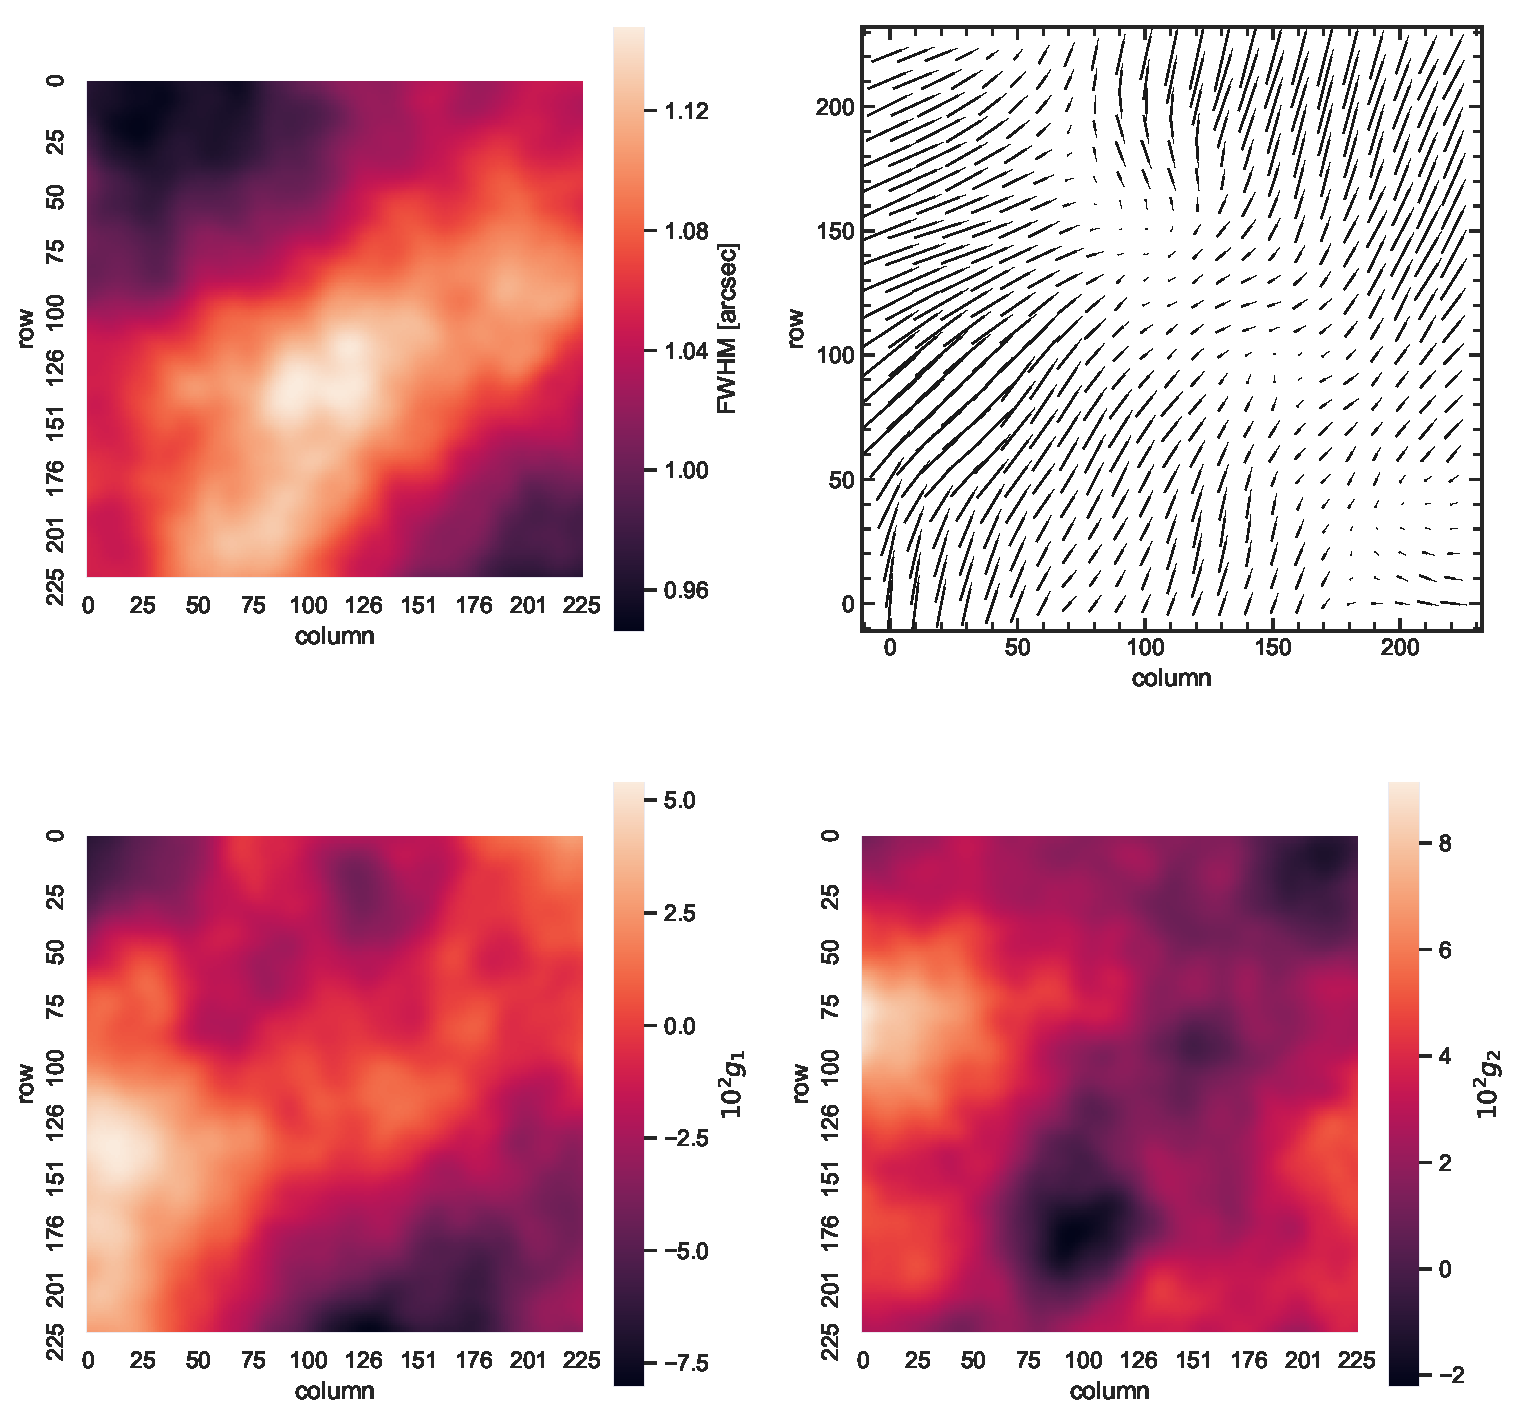
\includegraphics[width=0.7\textwidth]{figures/pspsf.pdf}
        \caption{
            Variable PSF model statistics for a DECam-like exposure. The top-left
        panel shows the variation in the FWHM in arcseconds. The top-right panel
        shows a visualization of the PSF ellipticity variation. The bottom-left panel shows
        the variation in the $1$-component of the PSF ellipticity. The bottom-right panel
        shows the variation in the $2$-component of the PSF ellipticity. The variation in
        this model is $\gtrsim10\times$ larger than the typical PSF variation for
        either DECam or expected LSST observations. The pixel scale is 0.263 arcsec
        so that each panel is approximately 1 arcmin on a side.
        \label{fig:pspsf}}
    \end{center}
\end{figure*}

\begin{figure}
    \begin{center}
        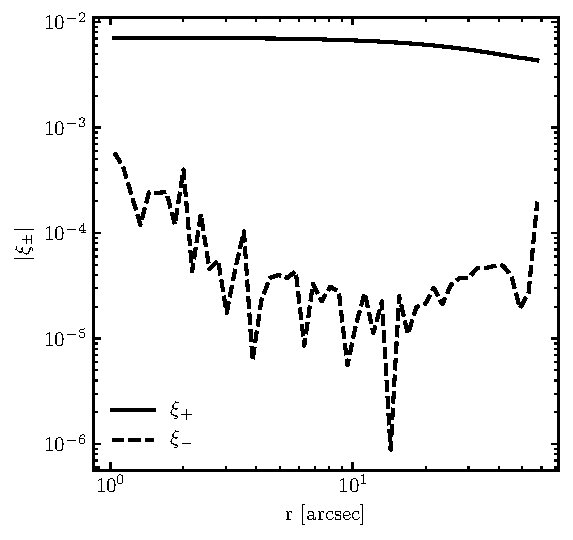
\includegraphics[width=\columnwidth]{figures/psxi.pdf}
        \caption{
            Variable PSF model shear correlation functions for a DECam-like exposure. LSST
        is expected to have shear correlation function magnitudes around
        $\sim\!10^{-4}$ \citep{jee2011}.
        \label{fig:psxi}}
    \end{center}
\end{figure}




%\bsp
%\label{lastpage}
\end{document}
